%% статьи в формате LaTeX для сборника статей "Системное         **
%% **  программирование".                                                   **
%% **  СПбГУ, мат.-мех. факультет, НИИ ИТ, 2005 г.                          **
%% **  Текст собирается с помощью программы latex                           **
%% **                                                                       **
%% ***************************************************************************

\documentclass[a5paper]{article}
\usepackage[a5paper, top=17mm, bottom=17mm, left=17mm, right=17mm]{geometry}
\usepackage[T2A]{fontenc} 
\usepackage[utf8]{inputenc}
\usepackage[english,russian]{babel}
\usepackage{graphicx}
\usepackage{indentfirst}
\usepackage{hyperref}



\sloppy
\pagestyle{empty}

%% ***************************************************************************
%% **                                                                       **
%% **  Место для названия статьи                                            **
%% **                                                                       **
%% ***************************************************************************
\title{Синтаксический анализ регулярных множеств}

%% ***************************************************************************
%% **                                                                       **
%% **  Место для авторов, их email-адресов и названий институтов            **
%% **                                                                       **
%% ***************************************************************************
%\author{С.В.Григорьев\\
%rsdpisuy@gmail.com\\
%\and Санкт-Петербургский государственный университет\\
%198504, Университетский проспект, 28, Старый Петергоф,\\
%Санкт-Петербург, Россия}
%\date{}
\begin{document}

%\maketitle
%\thispagestyle{empty}

%% ***************************************************************************
%% **                                                                       **
%% ** Аннотация                                                             **
%% **                                                                       **
%% ***************************************************************************
%\begin{quote}

%\renewcommand{\thefootnote}{}

%% ***************************************************************************
%% **                                                                       **
%% ** Авторские права                                                       **
%% **                                                                       **
%% ***************************************************************************
%\setcounter{footnote}{0}
%\end{quote}

%% ***************************************************************************
%% **                                                                       **
%% ** Текст статьи                                                          **
%% **                                                                       **
%% ***************************************************************************
\section*{---}

Предполагаемую структуру свёртки можно описать КС-грамматикой. При этом можно использовать более выразительные конструкции, чем нормальная форма Хомского.

\begin{itemize}
    \item Регулярные выражения
        \begin{verbatim}
    any : (A | U | G | C)+ // любой из символов {A,U,G,C} не менее 1 раза
        \end{verbatim}
    \item \textbf{Повторения} позволяют ограничивать количество однотипных элементов (в отличии от +*). 
        \begin{verbatim}
     s : any*[2..5] // повторение any от 2 до 5 раз включительно
        \end{verbatim}
    \item Метаправила
        \begin{verbatim}
    not_empty_list<item sep>: item (sep item)*
    s1: not_empty_list<NUM COLON>
    s2: not_empty_list<s1 DOT>
        \end{verbatim}
\end{itemize}

Возможный пример описания свёртки для tRNA.

\begin{verbatim}
[<Start>]
folded: stem<(a3 stem<a10> a3 stem<a7> a5 stem<a7> a2)>

stem<s>: 
      [0.24999975] (A stem<s> U)
    | [0.24999975] (U stem<s> A)
    | [0.24999975] (C stem<s> G)
    | [0.24999975] (G stem<s> C)
    | [0.24999975] (G stem<s> U)
    | [0.24999975] (U stem<s> G)
    | [0.000001] (s)

a1: [0.24999] (A)
  | [0.24999] (U)
  | [0.24999] (G)
  | [0.24999] (C)
\end{verbatim}

\begin{itemize}
\item \texttt{A B C D} --- терминалы, атомы входных цепочек
\item \texttt{any, simple1, simple2, s} --- нетерминалы
\item \texttt{s} -- стартовый нетерминал
\end{itemize}

Далее, можно искать всё, что совпадает с таким шаблоном, отбирать более вероятные.


Можно пытаться восстанавливать грамматики из известных структур свёрток, можно описывать их руками.

Далее, можно отдельно оценивать деревья. Например, на схожесть с уже известными.
\begin{figure}[H]
    \begin{center}
        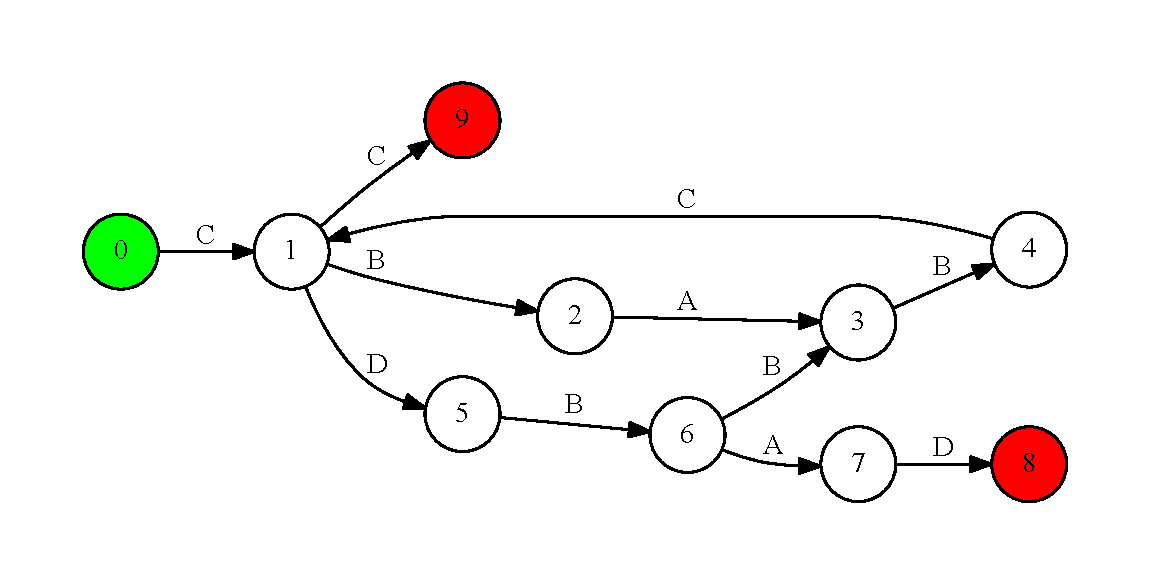
\includegraphics[width=11cm]{input.pdf}
        \caption{Входной граф}
        \label{pic1}        
    \end{center}
\end{figure}

Отдаём эту грамматику и граф нашему тулу. Он строит некую структуру, из которой можно понять, например, что он нашёл следующие вхождения (надеюсь, я ничего не пропустил).

\begin{figure}
    \begin{center}
        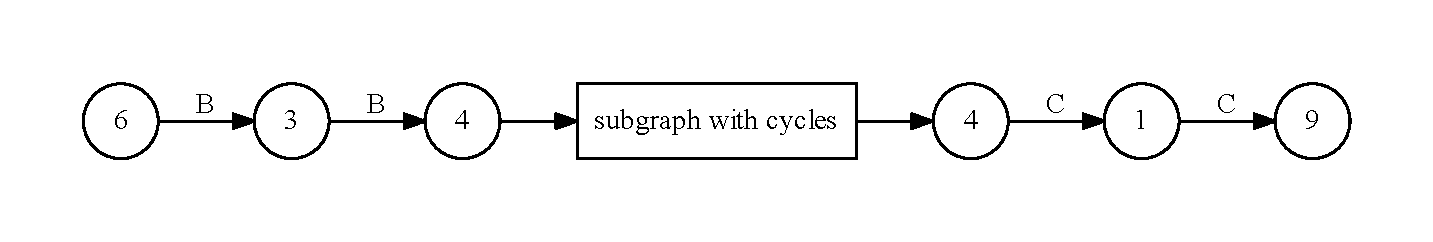
\includegraphics[width=11cm]{out1.pdf}
        \caption{Вхождение 1}
        \label{pic1}        
    \end{center}
\end{figure}

\begin{figure}
    \begin{center}
        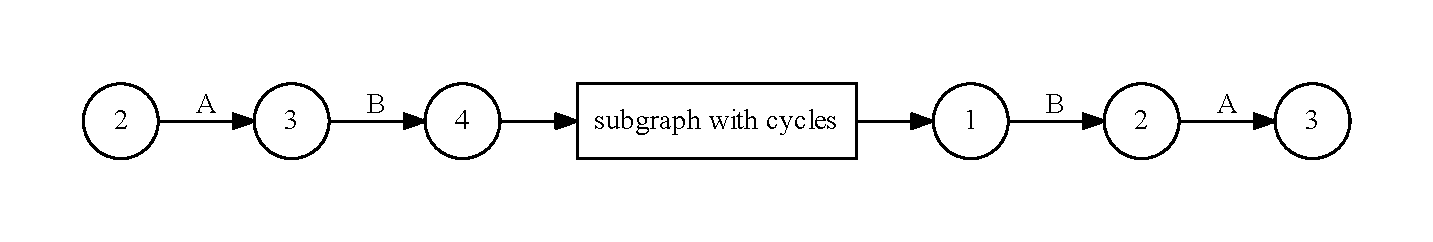
\includegraphics[width=11cm]{out2.pdf}
        \caption{Вхождение 2}
        \label{pic1}        
    \end{center}
\end{figure}

\begin{figure}
    \begin{center}
        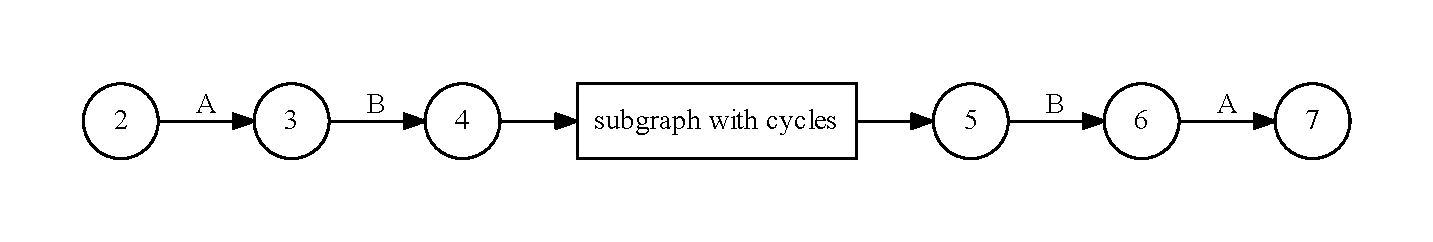
\includegraphics[width=11cm]{out3.pdf}
        \caption{Вхождение 3}
        \label{pic1}        
    \end{center}
\end{figure}


%% ***************************************************************************
%% **                                                                       **
%% ** Список литературы                                                     **
%% **                                                                       **
%% ***************************************************************************
%\begin{thebibliography}{99}
  
%\bibitem{RelaxedLALR}
%\emph{Ефимов А.А., Кириленко Я.А.} Построение ослабленного LALR-транслятора на основе анализа грамматики на избыточность // Системное программирование. Т. 4, вып. 1, 2009. С. 79--103.  


%\end{thebibliography}

\end{document}
